%----------------------------------------------------------------------------
\chapter{Case Study}\label{sect:case-study}
In this chapter I want to demonstrate the functionalities of Model-based test generation. For this I have created sample system, which models a garage gate. First I describe the common functionality of this system, then I set-up the system requirements and finally I introduce the implementation and design decisions of the system for different model-based testing tools.

\section{System introduction}
This garage gate software system consists of 6 different units (see figure \figref{overalBDD}): a gate, a lamp, a remote Controller, a control logic, motion sensor, a motor and a gate closed-state detection sensor.

\begin{figure}[!ht]
	\centering
	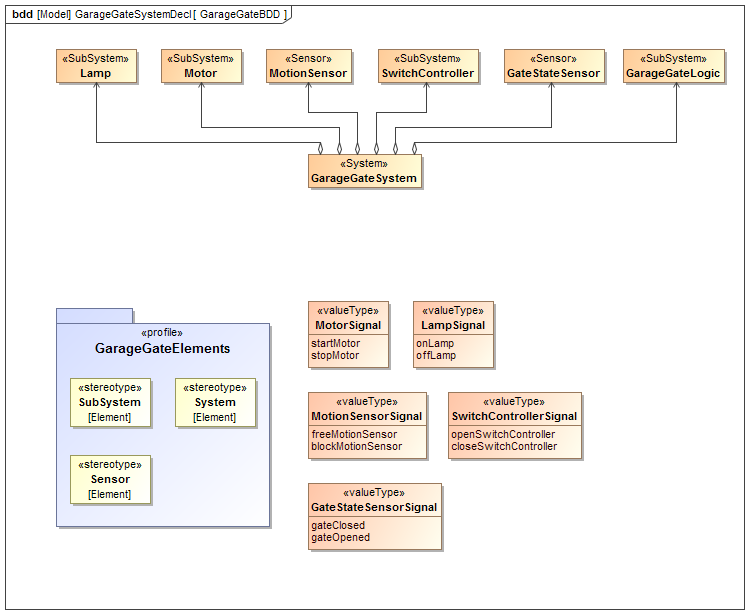
\includegraphics[width=100mm, keepaspectratio]{figures/magicDraw/bdd__GarageGateBDD.png}
	\caption{Garage system components and signals}
	\label{fig:overalBDD}
\end{figure}

First with the control switch we can simply send an action to the control logic that open or close the gate. If someone or something suddenly appears in the way of the gate, while it is moving, the movement stops. The motion sensor detects this interruption (the gate is blocked) or free status (the gate has free way). Before restarting the closing action, the control unit waits 5 seconds for the lighting warning. When the gate is finally closed, an additional sensor gives us plausibility for the gate physically closed state.

%TODO check the requirements
\iffalse
\section{Software Requirements}
\subsection{Gate}
\begin{description}
	\item[Req-01-1] The 
\end{description}
\fi

\subsection{Lamp}
\begin{description}
	\item [REQ-02-1] The lamp lighting frequency should be 1 second.
	\item [REQ-02-2] One lighting section is 5 seconds long.
\end{description}

\subsection{Remote Controller}
\begin{description}
	\item [REQ-03-1] The controller should have an open and a close gate action button.
	\item [REQ-03-2] One action must be completely finished to start a new action. 
	\item [REQ-03-3] When the battery is low, the remote controller should warn this to the control logic. %necessary?
\end{description}

\subsection{Control Logic}
\begin{description}
	\item [REQ-04-1] The \textit{Control Logic} can get new actions from the \textit{Remote Controller}, while no other action is being processed.
	\item [REQ-04-2] While the gates are moving (by an action from the \textit{Remote Controller}), the \textit{Control Logic} should stop the movement, if it gets a \textit{blocking} sign from the \textit{Motion Sensor}. Consequently the \textit{Control Logic} should continue the movement, it it gets a \textit{free} sign from the \textit{Motion Sensor}.
	\item [REQ-04-3] The \textit{Control Logic} can receive the signals from the \textit{Motion Sensor}, \textit{Lamp}, \textit{Remote Controller}
	\item [REQ-04-4] While the \textit{Lamp} is lighting the gates should not move.
\end{description}

\subsection{Motion Sensor}
\begin{description}
	\item [REQ-05-1] The sensor must detect if anything is between the two pillars of the gate. 
	\item [REQ-05-2] If the sensor detect blocking thing in the gate, a \textit{blocking} signal must be sent immediately to the \textit{Control Logic}.
	\item [REQ-05-3] If the sensor can not detect anything between the two gates, a \textit{free} signal must be sent to the \textit{Control Logic}
	\item [REQ-05-4] When the sensor detects free status after the blocking status, there must be at least 3 seconds until the first \textit{free} signal can be sent to the \textit{Control Logic}.
\end{description}

\subsection{Motor}
\begin{description}
	\item [REQ-06-1] 
	\item [REQ-06-2] 
	\item [REQ-06-3] 
\end{description}


%TODO write design details
\section{System model representation}
%specific UML diagrams, component diagram or component composition diagram (like SWSV::RIS description)

First I want to model the physical representation of the sample on the \figref{GarageBDD} figure.

The system consists 5 elements:
\begin{itemize}
	\item Lamp: This component is represents the lamp itself.
	\item Motor: This block can move the gates to opened and closed state.
	\item MotionSensor: These sensors are on the two pillars of the gate, and detect if something is in between of these sensors.
	\item SwitchController: This block is for the remote controller physical realization.
	\item GarStateSensor: The sensor which is detects the actual state of the gate.
    \item GarageGateLogic: This involves the safety logic and the gives control messages to the blocks.
\end{itemize}

\begin{figure}[!ht]
	\centering
	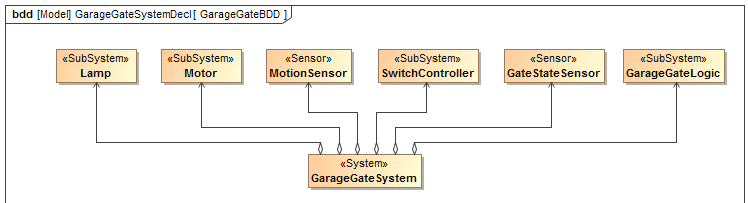
\includegraphics[width=100mm, keepaspectratio]{figures/magicDraw/bdd__GarageGateBDDcut.png}
	\caption{Garage system physical components}
	\label{fig:GarageBDD}
\end{figure}

The \figref{GateLogicComm} figure introduce the communication between the above listed blocks. We can say that each block is connected to one master block, who is the GarageGateLogic with specific ports.

\begin{figure}[!ht]
	\centering
	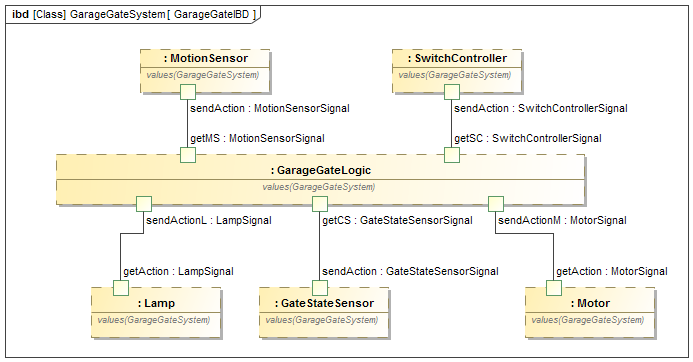
\includegraphics[width=150mm, keepaspectratio]{figures/magicDraw/ibd__GarageGateSystem__GarageGateIBD.png}
	\caption{Gate controller internal block diagram}
	\label{fig:GateLogicComm}
\end{figure}

A garage gate fundamentally have 2 main states, the \textit{Opened} and \textit{Closed} states, which is shown below on \figref{Garage Statemachine} figure. First of all we can start from the initial \textit{Closed} state, where we can open the gate with an 'open' command. This command sets the state machine in an \textit{Opening} state, while starting the motor functions. While opening the gate, somebody or something can move into the way, so this becomes \textit{Block Opening}. The gate is opening again, if the blocking object moved out of the way consequently it is free. After the \textit{Opening} phase succeeded the gate is \textit{Opened}. 

In this state we can 'close' the gate with a simple command by the \textit{Switch Controller}, and the state machine goes to the \textit{Closing} state. There could be also a blocking action, which stops the closing movement. From this state the gate is starting the closing movement again after a few seconds \textit{Lighting}. When the closing action finished the gate is \textit{Closed} and the motor has been stopped.

\begin{figure}[!ht]
\centering
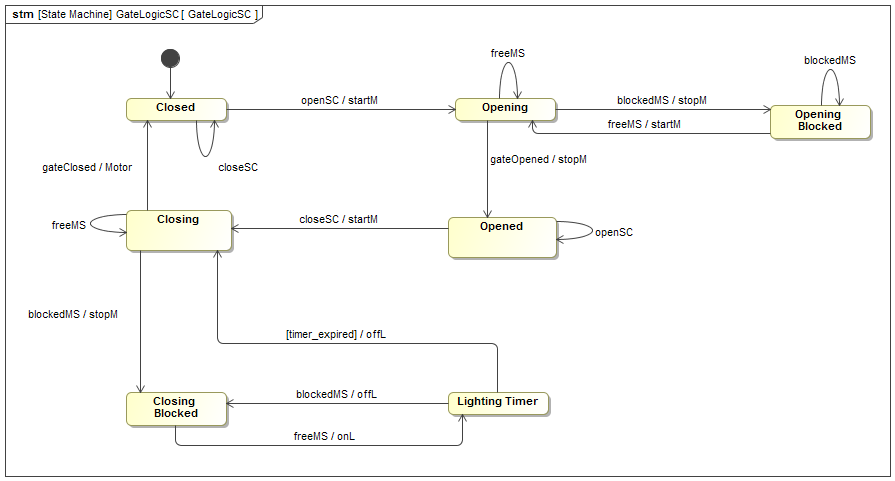
\includegraphics[width=150mm, keepaspectratio]{figures/magicDraw/GateLogicSC.png}
\caption{Garage gate state machine diagram}
\label{fig:Garage Statemachine}
\end{figure}

%TODO define what testing scenarios i will use
\paragraph{Testing goals}
The tests should achieve all the possible states of the SUT, because we want to detect the behaviour of the SUT in all use cases.

\section{Implementation}

\section{Testing results}
\subsection{GraphWalker}

\subsection{SpecExplorer}